\documentclass[11pt,letterpaper]{article}
\pdfoutput=1
\usepackage{jheppub}

\usepackage[utf8]{inputenc}

\usepackage{color}
\usepackage{graphicx}
\usepackage{tabularx}
\usepackage{xspace}

\usepackage{verbatim}
\usepackage{amsmath}
\usepackage{amssymb}
\usepackage[caption=false]{subfig}
\usepackage{url}
\usepackage{bbold}
\usepackage{slashed}
\usepackage{array}
\usepackage{hepunits}

\usepackage{multirow}
\usepackage{threeparttable}
\usepackage{paralist}

%\newcommand{\GeV}{\text{GeV}}
%\newcommand{\TeV}{\text{TeV}}
\newcommand{\SO}{\text{SO}}
\newcommand{\SU}{\text{SU}}
\newcommand{\SM}{\text{SM}}

\newcommand{\U}{\text{U}}
\newcommand{\CKM}{\text{CKM}}
\newcommand{\eff}{\text{eff}}

\newcommand{\genang}[2]{{\lambda^{#1}_{#2}}}


\newcommand{\ev}{\text{event}}
\newcommand{\jet}{\text{jet}}
\newcommand{\jets}{\text{jets}}
\newcommand{\subj}{\text{subjet}}
\newcommand{\subjs}{\text{subjets}}
\newcommand{\cut}{\text{cut}}
\newcommand{\trim}{\text{trim}}
\newcommand{\Ecut}{E_{{\rm cut}}}

\newcommand{\ptc}{p_{T{\rm cut}}}
\newcommand{\ptsubc}{p_{T{\rm subcut}}}

\newcommand{\sub}{\text{sub}}
\newcommand{\miss}{\text{miss}}

\newcommand{\pythia}{\textsc{Pythia~8}\xspace}
\newcommand{\herwig}{\textsc{Herwig++}\xspace}
\newcommand{\eventtwo}{\textsc{Event2}\xspace}
\newcommand{\vincia}{\textsc{Vincia}\xspace}
\newcommand{\sherpa}{\textsc{Sherpa}\xspace}

\newcommand{\FastJet}{\textsc{FastJet}\xspace}
\newcommand{\MadGraph}{\textsc{MadGraph}\xspace}

\newcommand{\df}{\text{d}}
\newcommand{\vev}[1]{\langle #1 \rangle}


\DeclareRobustCommand{\Sec}[1]{Sec.~\ref{#1}}
\DeclareRobustCommand{\Secs}[2]{Secs.~\ref{#1} and \ref{#2}}
\DeclareRobustCommand{\Secss}[3]{Secs.~\ref{#1}, \ref{#2}, and \ref{#3}}
\DeclareRobustCommand{\App}[1]{App.~\ref{#1}}
\DeclareRobustCommand{\Tab}[1]{Table~\ref{#1}}
\DeclareRobustCommand{\Tabs}[2]{Tables~\ref{#1} and \ref{#2}}
\DeclareRobustCommand{\Fig}[1]{Fig.~\ref{#1}}
\DeclareRobustCommand{\Figs}[2]{Figs.~\ref{#1} and \ref{#2}}
\DeclareRobustCommand{\Figss}[3]{Figs.~\ref{#1}, \ref{#2}, and \ref{#3}}
\DeclareRobustCommand{\Eq}[1]{Eq.~(\ref{#1})}
\DeclareRobustCommand{\Eqs}[2]{Eqs.~(\ref{#1}) and (\ref{#2})}
\DeclareRobustCommand{\Eqss}[3]{Eqs.~(\ref{#1}), (\ref{#2}), and (\ref{#3})}
\DeclareRobustCommand{\Ref}[1]{Ref.~\cite{#1}}
\DeclareRobustCommand{\Refs}[1]{Refs.~\cite{#1}}

\newcommand{\be}{\begin{equation}}
\newcommand{\ee}{\end{equation}}
\newcommand{\nn}{\nonumber}

\renewcommand{\textfraction}{0.10}
\renewcommand{\topfraction}{0.90}
\renewcommand{\bottomfraction}{0.90}
\renewcommand{\floatpagefraction}{0.65}

%% Reference commands %%
\newcommand{\mb}[1]{\boldsymbol{#1}}
\newcommand{\bm}[1]{\boldsymbol{#1}}
\newcommand{\mbo}[1]{\boldsymbol{\overline{#1}}}

\usepackage{xspace}


\def\Tr{\mathop{\rm Tr}}
\newcommand{\rep}[1]{\mathbf{#1}}
\newcommand{\conjrep}[1]{\overline{\mathbf{#1}}}


\renewcommand{\a}{\alpha}
\renewcommand{\b}{\beta}
\newcommand{\e}{\epsilon}
\newcommand{\D}{\Delta}
\renewcommand{\l}{\lambda}
\renewcommand{\th}{\theta}
\newcommand{\bq}{\bar{q}}
\newcommand{\zcut}{z_{\rm cut}}

\newcommand{\IZ}{\mathbb{Z}}
\newcommand{\cD}{\mathcal{D}}
\newcommand{\cL}{\mathcal{L}}
\newcommand{\cR}{\mathcal{R}}
\newcommand{\cF}{\mathcal{F}}
\newcommand{\cI}{\mathcal{I}}
\newcommand{\cK}{\mathcal{K}}
\newcommand{\beq}{\begin{eqnarray}}
\newcommand{\eeq}{\end{eqnarray}}

\newcommand{\F}{\mathcal{F}}
\newcommand{\Ft}{\widetilde{\mathcal{F}}}
\newcommand{\G}{\mathcal{G}}
\newcommand{\Gt}{\widetilde{\mathcal{G}}}
\newcommand{\HH}{\mathcal{H}}
\newcommand{\HHt}{\widetilde{\mathcal{H}}}
\newcommand{\ord}[1]{\mathcal{O}\!\left(#1\right)}

\newcommand*\numcircledmod[1]{#1 \!\!\! \bigcirc}

\newcommand{\Njet}{\widetilde{N}_{\rm jet}}
\newcommand{\dN}[1]{\Delta_{#1}}
\newcommand{\dNpm}{\Delta_{2\pm}}
\newcommand{\dNp}{\Delta_{2+}}
\newcommand{\dNm}{\Delta_{2-}}
\newcommand{\dNtm}{\Delta_{3-}}

\newcommand{\cT}{\mathcal{T}}
%\newcommand{\as}{\alpha_s}
\renewcommand{\angle}{\theta}

%\definecolor{darkgreen}{rgb}{0,0.5,0}
%\newcommand{\jdt}[1]{\textbf{\textcolor{darkgreen}{(#1 --jdt)}}}
%\newcommand{\gs}[1]{\textbf{\textcolor{darkblue}{(#1 --gs)}}}

\definecolor{mildred}{rgb}{0.8,0,0}
\newcommand{\info}[1]{\textbf{\textcolor{mildred}{(#1)}}}


\begin{document}


\title{Towards Extracting the Strong Coupling Constant \\ from Jet Substructure at the LHC}

\author[a]{Disha Bhatia?,}
\author[a]{Grigorios Chachamis,}
\author[a]{Suman Chatterjee?,}
\author[a]{Frederic Dreyer,}
\author[a]{Maria Vittoria Garzelli,}
\author[a]{Philippe Gras,}
\author[a]{Andrew Larkoski,}
\author[a]{Daniel Maitre,}
\author[a]{Simone Marzani, }
\author[a]{Ian Moult,}
\author[a]{Ben Nachman,}
\author[a]{Andrzej Siodmok,}
\author[a]{Andreas Papaefstathiou,}
\author[a]{Peter Richardson,}
\author[a]{Tousik Samui,}
\author[a]{Gregory Soyez,}
\emailAdd{gregory.soyez@cea.fr}
\author[a]{and Jesse Thaler}
\emailAdd{jthaler@mit.edu}

\affiliation[a]{Les Houches}

\abstract{YADA}

\maketitle

%%==============
\section{Introduction}
%%==============

\info{Ben, Ian, Jesse, Grigorios, Maria}

Goal of jet substructure community

Application of new techniques beyond tagging

AIM:  Achieve something like 10\% precision to start to answer other questions

\subsection{Cite Dump}

PDG \cite{Olive:2016xmw}

mMDT \cite{Dasgupta:2013ihk,Dasgupta:2013via}

filtering/pruning/trimming \cite{Butterworth:2008iy,Ellis:2009su,Ellis:2009me,Krohn:2009th}

Soft Drop \cite{Larkoski:2014wba}

Cambridge/Aachen \cite{Wobisch:1998wt,Dokshitzer:1997in}

Calculation 1 \cite{Frye:2016okc,Frye:2016aiz}

Calculation 2 \cite{Marzani:2017mva}

AKT \cite{Cacciari:2008gp}, FastJet \cite{Cacciari:2011ma}

Boost Reports \cite{Abdesselam:2010pt,Altheimer:2012mn,Altheimer:2013yza,Adams:2015hiv}

Sudakov Safety \cite{Larkoski:2013paa,Larkoski:2015lea}, $z_g$ \cite{Larkoski:2015lea}

\begin{figure}
\begin{center}
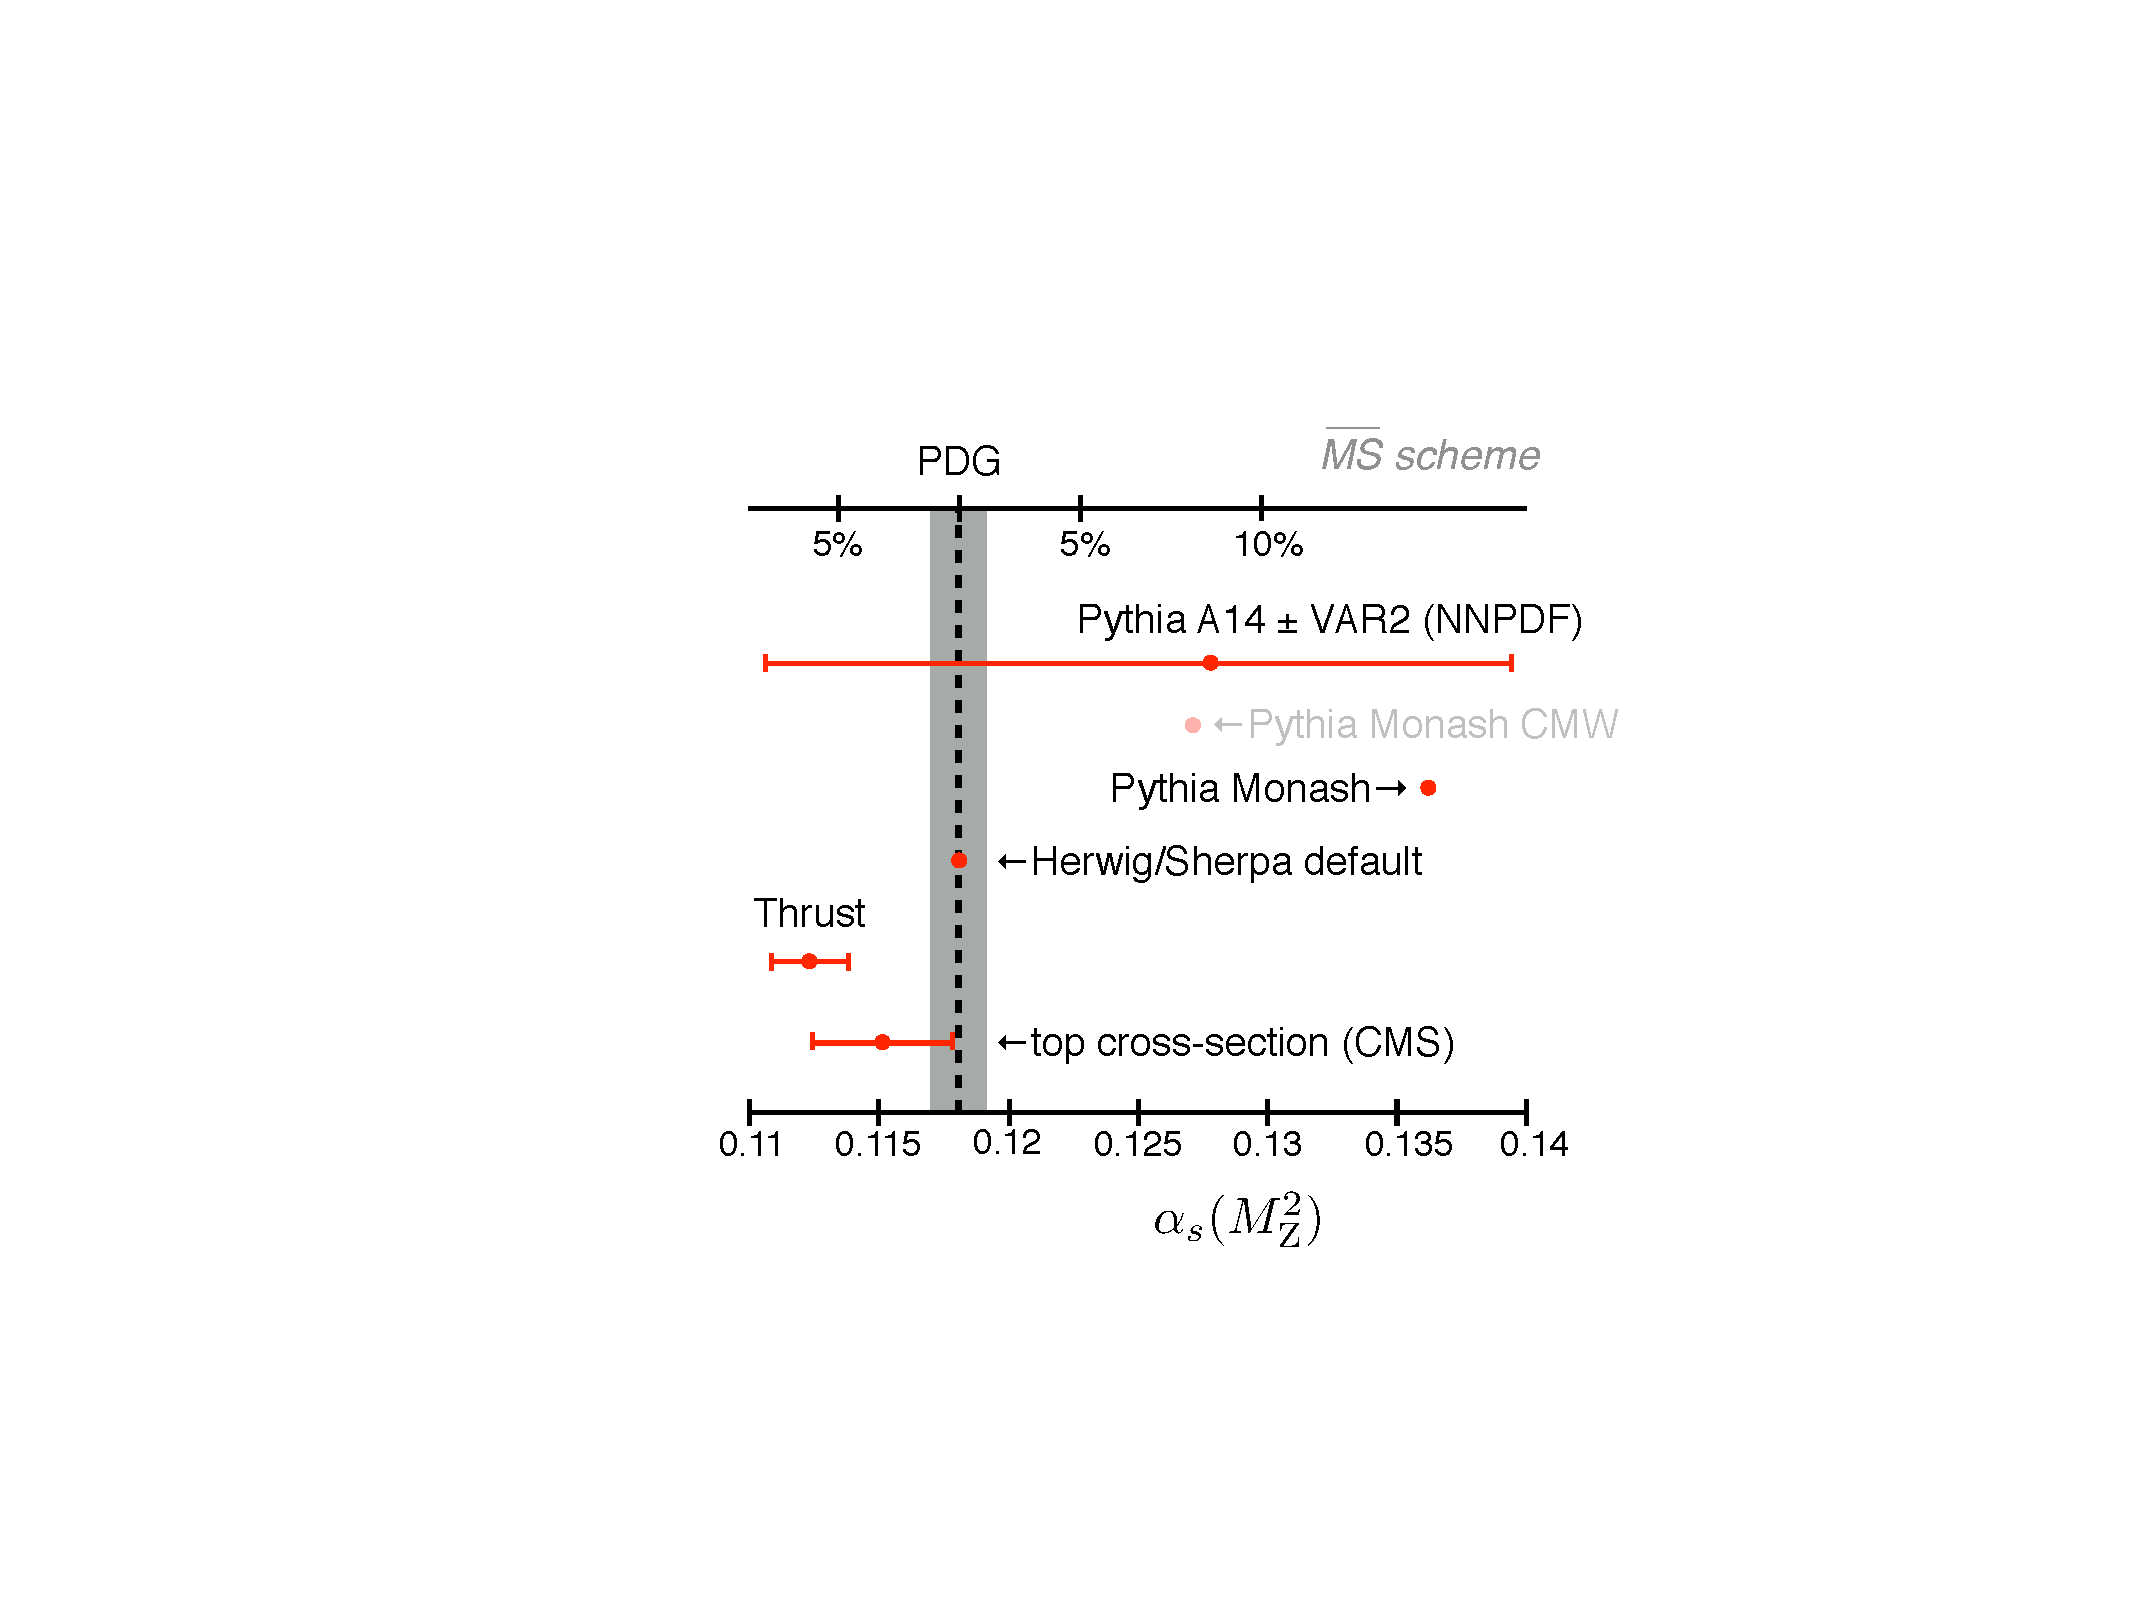
\includegraphics[width = 0.6\columnwidth]{figures/alphas_propaganda.pdf}
\end{center}

\caption{Ben's propaganda plot}

\label{fig:propaganda}

\end{figure}

%%==============
\section{Grooming Away Soft Complications}
\label{sec:softcomplications}
%%==============

\info{Andrew, Simone}


Generic result of grooming is removing wide-angle soft radiation.  What impact does this have?

\subsection{Mitigating Nonperturbative Effects (e+e- and pp)}

\begin{itemize}
\item grooming original purpose: reduce sensitivity to soft-wide angle radiation
\item it obviously reduces the impact of UE and pile-up in pp collision
\item what about hadronization? at first sight less obvious because we get rid of soft radiation but we also reduce the effective radius. Competing effects?
\item however it helps with hadronization too: parametric understanding (here there is some calculation in mMDT paper and Harvard paper too). Some unpublished studies exist on  for $\beta>0$ by Gregory, Lais and SM. 
\item Abundant MC evidence that helps
\item Open question: any deeper understanding in terms of shape functions?
\end{itemize}

Comparison to shape function in thrust.  Grooming gives different sensitivity to NP effects.

In standard thrust fits, whole distribution shifts from NP.  Degenerate with $\alpha_s$ shift, hard to disentangle.

Grooming pushes NP effects to separate region.  Separation of NP region, resummation region, fixed order regime (at high enough jet $p_T$).

\subsection{Process Independence at Hadron Colliders (pp)}
clearly there still is some process-dependence, in terms of q/g fractions as well as hard coefficients. It is however much reduced.
compare to issue of PDF, 3-jet over 2-jet, ECF extractions
Grooming removes soft correlations: it ``turns the LHC into an e$^+$e$^-$ machine (too strong?)
Related:  Grooming remove NGLs and other contamination. It makes things easier to calculate. 


\subsection{Improved Detector Resolution (LHC)}

Cites to pileup study.

Grooming needed to help pileup from LHC


%%==============
\section{Case Study: Groomed Jet Mass}
%%==============

\info{Andrew, Simone}

Soft drop mass is most accurate jet substructure observable to date.  Review soft drop, and current calculations

\subsection{Soft Drop Declustering}

Review of soft drop

\subsection{Method 1 (name?) Analytic Calculation}

Andrew, et al.

\subsection{Method 2 (name?)  Analytic Calculation}

Simone and Gregory, et al.

(calculated at NNLL, good enough to start extraction)

\subsection{Concrete Benefits of Grooming}

Show that grooming does what's advertised in \Sec{sec:softcomplications}.

%%==============
\section{Idealized Performance at the LHC}
%%==============

\info{Ben, Andrzej, Jesse, Gregory, Grigorios, Frederic}

\subsection{Extraction of Theory Templates}

	Theory Templates.

	Ben is doing this.

	Current best NNLO + NLO for dijets, but for time, drop both first Ns
 
 Can do NLO + LO on days timescale (even if theory uncertainty is too large)

 Right now, assume known quark/gluon function, relax later.


\subsection{Estimate of Experimental Resolution}

	Parametrized Experimental Resolution?

	Ben has a toy simulation
	Resolution achievable, uncertainty?
	How to we think this will be done in this study (can we use fast simulation, or parametrization?)
	Statistical uncertainties at high pT?
	Pileup:  there are studies of this with current level of pileup, not a big deal yet

	Uncertainty worse at low and high mass, need to derive parametrized uncertainty
	
	Trade off with pT (rate versus NP control)


\subsection{Fit in Pure Quark/Gluon Samples}

Fit Methodology:
	Which fix range (minimizing theory and experimental uncertainties)?
	Constraining quark vs gluon fraction (varying SD parameters)?
	Zeroth-order feasibility study
	
	Plot is for distribution folded over PDFs (can we get rid of that?)

	Choice of jet radius (varying resummation scale)

Assume (for this section) limited by experimental uncertainties



\subsection{Constraining Quark/Gluon Fraction with Data}

	Question:  constrain quark/gluon fraction (adjust $z_cut$)?
	Need to decide beta and zcut values
	Need to matching to fixed order
	beta = 0 mass is baseline
	
	
	Another study to mitigate quark/gluon fraction uncertainties
	Sensitivitity to PDF only to the extent of getting quark/gluon fraction
	Can mitigate that with fit.




%%==============
\section{Assessing Theoretical Uncertainties}
%%==============

\info{Simone, Andrew, Frank, Ian, Gregory, Frederic}

Above analysis was with no (or small uncertainties).  What are leading uncertainties?  Estimate.

\subsection{Perturbative Scale Variations}

	Understanding scales at which $\alpha_s$ is being probed (as a function of zcut and beta)
		3-jet / 2-jet probes TeV
		But jet shapes probe lower scale than scale of the jet (which scale)?

	Perturbative Scale Variation (NLL/NNLL)


\subsection{Nonperturbative Effects from Shape Function}

	Treat NP effects (shape function?)  	Do we need shape function (or just a cut value)?

	Need to think about $\Omega_0$ issue (is it a shape-function-like shift?  Or just parametrically correct?)


\subsection{Finite $z_{\rm cut}$ Corrections}

	Finite zcut effects.  resummation vs.  power corrections?

\subsection{Fixed-Order Corrections}

	Matching to fixed-order?
		Universality in resummation region...
		...but process-dependence in fixed order region
		Efficiency of matching using NLO, making grid is painful
		Get help from FOMC expert
		LO matching is tree-level, e.g. MadGraph, PDFs...
		Matching to Fixed Order (remove the region from the fit, or figure out efficient calculations strategy.)

	Does peak give $\alpha_s$ information?
	
\subsection{Sensitivity to Initial State Effects }

	Parton Distribution Functions, 	Initial State Radiation, Underlying event.




%%==============
\section{Alternative Observables}
%%==============

\info{Gregory, Jesse, Ian}

Beyond Soft Drop Mass?

\subsection{Additional Soft Drop Observables}

Angularities and $R_g$.

\subsection{Single-emission Observables}

Possible Dump this

\subsection{Track-based Observables}

Insensitivity to pileup, improved angular resolution.
	Tracking observables more sensitive




%%==============
\section{Estimated Sensitivity from Parton Showers}
%%==============


\info{Andrzej, Johannes, Maria, Frederic, Peter, Tousik}

Estimated Sensitivity in Parton Shower MC

Adjust $\alpha_s$ in the final state PS and see the fit (make sure you see the same thing)

\subsection{Samples}

	Use pure Z + quark, pure Z+ gluon, and  dijet
	
	MadGraph hard scattering, interfaced with Pythia/Herwig
	
	13 TeV
	PDF choice?  (default per generator, or from MadGraph)
	Parton-level in MadGraph Born-level ($p_t > 450~\GeV$)
	Start with 100k events.
	
	
	$pT > 500~\GeV$, anti-$k_t$ $R = 0.8$, $|eta| < 2.5$

	
	
	Measure Pythia $\alpha_s$  with Herwig?
	
	Observables in RIVET

\subsection{Observables}


Observables:
-- Baseline:  mMDT mass (zcut = 0.1, beta = 0)
-- Sweeps:  zcut = 0.05, 0.1, 0.2
-- beta = 0, 1, 2
-- Angularity:  alpha = 0.5, 1.0, 2.0
-- $R_g$
-- Plus track based
-- No single emission for this study

\subsection{Extracting Parton Shower Templates}

	Use templates, e.g. $\theta_g$ distirbution as a function $\alpha_s$


\subsection{Consistency Check for Soft Drop Mass}
	Compare to analytic or parton shower study (do a closure test)

	Try different ME matching prescriptions, see if they close

	Plot of $\alpha_s$ versus log likelihood (statistical ssensitivity)

\subsection{Test of Alternative Observables}

Make sure that you measuring something correlated with $\alpha_s$




%%==============
\section{Prospects at Lepton Colliders}
%%==============



\info{Jesse}

	Look at e+e- case of jet shapes there (no quark fraction issue)

	Make a statement on e+e- (LEP) as well (can it do better than thrust?)
		Probes lower scales, so still interesting

	Limit our scope to e+e- is an option, though could just be statement, no study

	If we do e+e-, has to be compared to thrust



%%==============
\section{Conclusions}
%%==============

\info{All}

\begin{acknowledgments}

The work of GS is supported in part by the Paris-Saclay IDEX under the
IDEOPTIMALJE grant, by the French Agence Nationale de la Recherche,
under grant ANR-15-CE31-0016, and by the ERC Advanced Grant Higgs@LHC
(No.\ 321133).
%
The work of JT is supported by the DOE under grant contract numbers DE-SC-00012567 and DE-SC-00015476.

\end{acknowledgments}

\bibliographystyle{jhep}
\bibliography{lh2017_alphas}

\end{document}
